\documentclass[a4paper,11pt]{article}
%\documentclass[a4paper,12pt]{article}
%\documentclass[11pt,a4paper,nocolor]{moderncv}
\usepackage[backend=biber,sorting=ydnt,maxnames=18,giveninits=true,labelnumber=true,defernumbers=true]{biblatex}
%\usepackage[backend=biber,sorting=ydnt,maxnames=18,giveninits=true]{biblatex}
%\usepackage[bibstyle=publist]{biblatex}
\usepackage{xstring}
\usepackage{url}
\usepackage{booktabs}
\usepackage{hyperref}

\usepackage{titlesec}
\titlespacing*{\section}{0pt}{6pt plus 1pt minus 0.5pt}{3pt plus 0.5pt}
%\titlespacing*{\subsection}{0pt}{5.5ex plus 1ex minus .2ex}{4.3ex plus .2ex}

\titlespacing*{\paragraph}
{0pt}{3pt plus 1pt minus 0.5pt}{3pt plus 2pt minus 0.5pt}

\usepackage{enumitem}
\setlist{nosep}

\usepackage{tcolorbox}

\usepackage{fontspec}
\setmainfont{Cambria}
\setsansfont{Calibri}

%\setlength{\itemsep}{0pt plus 1pt}
%\setlength{\itemsep}{0pt}
%\setlength{\topsep}{0pt}
\setlength{\parskip}{3pt plus 0.5pt minus 0.5pt}
%\setlength{\beforeskip}{3pt}


%\usepackage[scale=0.85]{geometry}
\usepackage[scale=0.85]{geometry}

\geometry{
 a4paper,
 total={170mm,257mm},
 left=20mm,
 top=20mm,
 }

\addbibresource{bib/varrodan.bib}
\addbibresource{bib/external.bib}
%\addglobalbib{bib/external.bib}

%\assignrefcontextkeyws[labelprefix=C]{C}
%\assignrefcontextkeyws[labelprefix=J]{J}

\renewcommand*{\mkbibnamegiven}[1]{%
\ifpartannotation{family}{self}{\textbf{#1}}{#1}}

\renewcommand*{\mkbibnamefamily}[1]{%
\ifpartannotation{family}{student}{#1\textsuperscript{*}}{%
\ifpartannotation{family}{self}{\textbf{#1}}{#1}}}

\usepackage{fancyhdr}
\pagestyle{fancy}\lhead{Research Statement} \rhead{May 2019}
\chead{{\bf Dániel Varró}} \lfoot{} \rfoot{\bf \thepage} \cfoot{}

\title{Research Statement}
\author{D\'aniel Varr\'o}
\date{May 2019}

\DeclareRefcontext{bref}{labelprefix=B}
\DeclareRefcontext{jref}{labelprefix=J}
\DeclareRefcontext{cref}{labelprefix=C}
\DeclareRefcontext{wref}{labelprefix=W}
\DeclareRefcontext{oref}{labelprefix=O}
\DeclareRefcontext{eref}{labelprefix=E}
\DeclareRefcontext{iref}{labelprefix=I}
%\DeclareRefcontext{extref}{labelprefix=X,sorting=none}
\DeclareRefcontext{extref}{sorting=none}
\DeclareBibliographyCategory{own}

\begin{document}
\maketitle

\setcounter{page}{20}


%\section{Summary of Excellence}
\begin{tcolorbox}[title=Summary of Excellence]
My research primarily focuses on providing \emph{precise and scalable techniques} and \emph{software tools} used for engineering critical software-intensive systems with a recent focus on \emph{smart and safe cyber-physical systems} (CPS) deployed over decentralized, heterogeneous platforms. As the leader of an excellent research team with 15 PhD and 25+ Masters students I supervised or co-supervised, we received \emph{7x Best/Distinguished Paper Awards} at major peer-reviewed conferences of software engineering. I also received \emph{two 10-year most influential papers} for past results achieved in my early career. My research papers received over 6570 citations yielding an h-index of 41. In the past 5 years, I was invited to deliver 6 keynote talks at international or national conferences or workshops, 10 talks at advanced schools, and 15+ talks at industrial events.

\vspace{3pt}

%\paragraph{A paragraph}
Moreover, I have actively contributed to turn \emph{novel research results and prototype tools} first into \emph{industrial strength open source frameworks} then \emph{to innovative services and products} maintained by IncQuery Labs, a successful Hungarian company co-founded with my former graduate students and used by major international companies.
% operating in the CPS domain.
\end{tcolorbox}

In this research statement, I first summarize the five most significant research contributions between 2000 and 2015, which already had impact, then I summarize recent lines of research from the last 5-6 years. Then, I will overview ongoing and prospective future lines of research. Finally, I present a summary of impact for three research papers written in different stages of my career.

\section{Past Research Contributions (2000-2015)}

\subsection{Context}

In the past decade, model-based systems engineering (MBSE) has become a key technique for designing critical systems in application domains like avionics or automotive \cite{Broy2012,Whittle2014}. MBSE facilitates the systematic use of models on various levels of abstraction from an early phase of the development process in order to simultaneously \emph{increase productivity and quality} while \emph{reducing development costs} by avoiding costly re-design cycles compared to detecting the same problem by traditional testing. 

%System requirements and initial design 
System design is captured by \emph{high-level engineering models} using modeling languages (like UML, SysML, AADL, Capella). These models enable to immediately check design rules and well-formedness constraints imposed by the underlying platform (such as AUTOSAR or ARINC653) to design flaws early. Early \emph{hidden formal analysis of system models} can be carried out by generating various mathematical models by automated model transformations (horizontal MTs) to detect and eliminate conceptual flaws and quality bottlenecks. Results of precise mathematical analysis are back-annotated to system models, thus systems engineers can observe and correct these problems using a formalism familiar to them. 

\begin{figure}[htb]
\centering
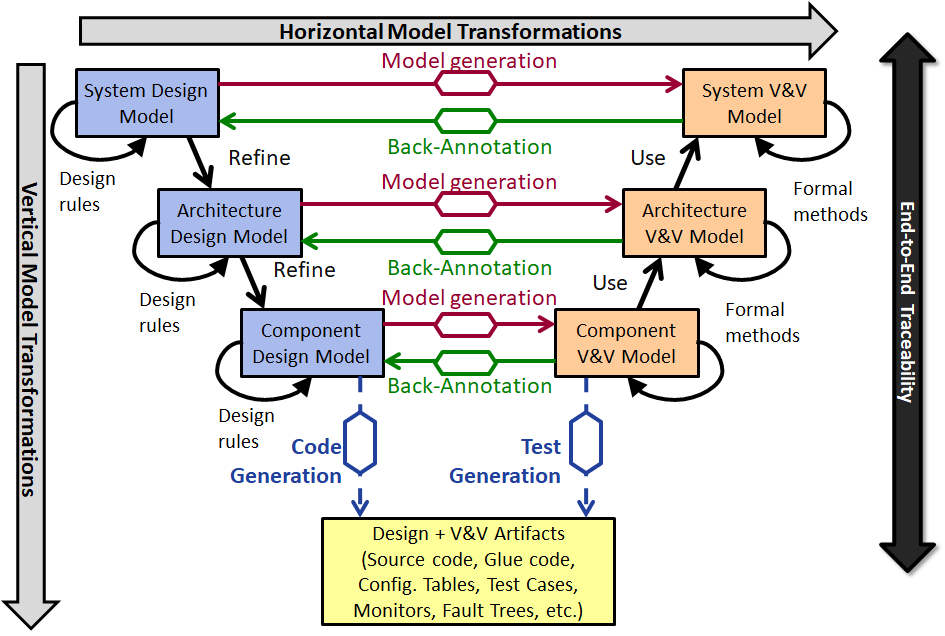
\includegraphics[width=.7\textwidth]{figures/mbse}
\caption{Models transformations in model-based systems engineering}
\label{fig:mbse}
\end{figure}


Automated code generators (also called vertical MTs) improve productivity by synthesizing provenly correct source code of a safety-critical application from a validated model \cite{Sturmer-TSE2007}. In addition to source code generation, MBSE tools can synthesize other design artifacts (such as configuration tables, fault trees, test cases, documentation) and provide support for end-to-end traceability \cite{Aizenbud-IBMSystems-2006}. MBSE changes the traditional V-model of systems engineering into a Y-model where certain certification artifacts are synthesized automatically from models of proven quality used at different levels of abstraction.

%\subsection{Summary}
Between 2000 and 2015, my research was characterized by (1) proposing novel, foundational concepts, (2) developing innovative and scalable techniques, (3) architecting and maintaining cutting edge prototype tools based on solid foundations, (4) continuously benchmarking and empirically evaluating these tools, and (5) using these results at design time in a wide range of applications in tools used for engineering critical systems (like avionics and automotive). 

\subsection{Scalable incremental model queries: Techniques and tools}

\paragraph{Result.}
With my students, G. Bergmann, M. Búr, Á. Hegedüs, Á. Horváth, G. Szárnyas, and I. Ráth, we developed highly scalable incremental techniques for continuously evaluating graph queries over large domain-specific instance models used in design and validation tools of critical systems. We turned scientific results \cite{models-2010-incquery,scp2015,models2014-iqd,icgt2015,sosym2016-viatra-invited,models2018-tool} into mature scalable software tools, which instantly re-evaluate validation rules over domain-specific graph models with millions of elements. 

\paragraph{Impact.}
The \href{https://www.eclipse.org/viatra/}{VIATRA open source project} has been actively \emph{used at large companies and research institutes} (e.g. Thales, Airbus, Ericsson, ThyssenKruppPresta, Embraer, NASA JPL), and in \emph{industrial modeling tools} (e.g. Papyrus, Capella, Artop). It provides the basis of \emph{innovative products} (\href{https://incquerylabs.com/incquery/}{IncQuery for MagicDraw, IncQuery Server}) developed at IncQuery Labs Ltd. It has been \emph{regularly used a baseline in performance comparisons} by leading researchers (e.g. D. Kolovos, J. Cabot, H. Giese). I \emph{delivered several keynote talks} on related topics at major scientific conferences and summer schools. Related papers \cite{models-2010-incquery,icmt2011,ase2011-tool,ecmfa2011,models2014-iqd,scp2015,icgt2015,sosym2016-viatra-invited,models2018-tool} have been cited over 400 times and \cite{models2018-tool} received a \textbf{Best Tool Paper Award} at the MoDELS 2018 conference. 

\paragraph{My role.}
All major contributors of the incremental graph query technology are my former PhD students. I have been the strategic leader of the research line until 2016 when the development of the open source framework was taken over by software engineers at IncQuery Labs Ltd, a high-tech company co-founded together with my former graduate students. This line of research has been funded by numerous projects: I was the site leader at BME of \emph{collaborative European projects} (e.g. SENSORIA, SecureChange), and the principal investigator (PI) of an ERC Starting Grant application (CERTIMOT) which went to the final round, but became out of budget, and later it received partial funding from the Hungarian Research Agency (ERC-HU). VIATRA technology received significant extra funding at IncQuery Labs, which is not detailed here. 


\subsection{Novel model transformations concepts}

\paragraph{Result.}
With my students, A. Balogh, Z. Balogh, G. Bergmann, Á. Hegedüs, Á. Horváth, I. Ráth, Z. Ujhelyi, we proposed novel model transformation concepts to capture mappings within and between various modeling languages. The scientific results provided foundations of the open source \href{https://www.eclipse.org/viatra/}{VIATRA} model transformation framework \cite{SCP2002,ASE2002,uml2004-meta,scp-2007,sosym2016-viatra-invited} which has been successfully developed along three generations since 2000. Novel concepts proposed by us for the first time include \emph{change-driven transformations} \cite{Rath-models09,sosym2011-cdt}, \emph{model transformation by example} (MTBE) \cite{models2006-varro,sosym2008-mtbe}, \emph{reactive transformations} \cite{icmt08-rbov08,icmt2015,sosym2016-viatra-invited} or \emph{model transformation slicing} \cite{ase2011-mtslice,icst2012}.

\paragraph{Impact.} 
In addition to the industrial use above, several papers on the VIATRA framework including \cite{SCP2002,ASE2002,uml2004-meta,models2006-varro,scp-2007,Bergmann-icmt09,Rath-sosym09,Rath-models09,Bergmann-sttt10} has been cited well over 2000 times. The paper \cite{uml2004-meta} got \textbf{a 10-year Most Influential Paper Award} at the IEEE/ACM MODELS 2014 conference, and I was invited to write an expert panel paper to the Software and Systems Modeling journal (Springer). Our first paper on change-driven transformations \cite{Rath-models09} received \textbf{Springer Best Paper Award} at IEEE/ACM MODELS 2009. The concepts of MTBE have been taken up by 12 independent research groups worldwide. I delivered \emph{several keynote talks} at international scientific conferences and summer schools on related topics.

\paragraph{My role.} 
The first generation of VIATRA was developed by myself in my PhD years, and I served as the strategic leader of the project until 2016. I was the main supervisor of 5 PhD students and co-supervisor of 2 PhD students in addition to 20+ MSc students doing research and development on related topics. Co-founding IncQuery Labs enabled to keep together the core team for 15 years by now. I was the principal investigator (PI) of three IBM Faculty Awards, and an ERC-HU Starting Grant application (see above) and the site leader of various \emph{collaborative European projects} (e.g. SENSORIA, SecureChange, MONDO) .

%My role in the related projects that funded this line of research is the same as in the previous line

\subsection{Performance benchmarks for model queries and transformations}
\paragraph{Result.}
Together with G. Varró and A. Schürr, we proposed the \emph{first performance benchmark for model transformation tools} in \cite{vlhcc05-vsv}. Since then, developing and maintaining performance benchmarks have been a focal topic of my research group. With my students, G. Bergmann, Á. Horváth, B. Izsó, G. Szárnyas, I. Ráth, Z. Ujhelyi, we systematically assessed the performance of various graph query technologies \cite{Bergmann-sttt10,scp2015,ttc2015,sosym2017-tb} for different technological platforms along the Train Benchmark. With researchers from University of Szeged, IncQuery was used for detecting anti-patterns in source code \cite{csmr2014,ist2015}.

\paragraph{Impact.} 
Our first paper \cite{vlhcc05-vsv} triggered a series of annual Transformation Tool Contests (over 12 editions) and it received a \textbf{Most Influential Paper Award} at IEEE VL/HCC 2016. Moreover, \cite{csmr2014} received the \textbf{Best Paper Award} at CSMR-WCRE 2014. The Train Benchmark \cite{ttc2015,sosym2017-tb} has been used by other researchers (e.g. D. Kolovos, X. De Carlos, G. Varró, G. Hinkel, H. Giese) for performance comparison from several independent research groups. Related papers have been cited over 275 times.

\paragraph{My role.} 
I was one of the three researchers who proposed the first ever benchmark for model transformations in 2005. Benchmarking was a focal topic of my PhD student G. Szárnyas, while many former students of mine (G. Bergmann, Á. Hegedüs, Á. Horváth, B. Izsó, I. Ráth, Z. Ujhelyi) made significant contributions to past benchmarking activities. I was a co-organizer of the first open transformation tool comparison as part of the AGTIVE 2007 conference \cite{agtive07-toolcontest}. I was the site leader at BME of the MONDO FP7 project and a collaborator of the MOGENTES FP7 project, which financed some of the related research activities.

\subsection{Rule-based guided design space exploration}

\paragraph{Result.}
Design space exploration (DSE) aims to derive design candidates fulfilling heterogeneous design constraints from an initial design sketch by applying a pre-defined set of operations. We proposed the concept of \emph{rule-based guided design space exploration} \cite{Horvath-models09,sosym2011-csp,ase2011-dse,ause2015,ase2014,mpm2014} to incorporate complex structural and consistency constraints frequently present in architecture models of automotive and avionics applications. The exploration process can be heuristically guided by hints obtained from the designer. DSE was applied to provide quick fixes in design environments built for business modeling \cite{vlhcc2011}. 

\paragraph{Impact.} 
Our paper \cite{ase2011-dse} at the IEEE ASE 2011 conference received an \textbf{ACM Distinguished Paper Award}. Other researchers (e.g. H. Vangheluwe, S. Zschaler and M. Wimmer) followed related lines of investigations building on our results. Key papers \cite{Horvath-models09,sosym2011-csp,ase2011-dse,ause2015,ase2014} received over 150 citations in total. The VIATRA-DSE open source software won \emph{two first prizes at the 9th Transformation Tool Contest} (TTC 2016). The prototype software was evaluated at NASA Jet Propulsion Lab for high-level mission planning.

\paragraph{My role.} 
DSE exploration served as a key research topic for three PhD students (Á. Horváth, Á. Hegedüs, A. Nagy) under my supervision. Global search-based techniques were developed in collaboration with H. Sahraoui and H. Abdeen \cite{ase2014} during my period as a visiting professor at Université de Montréal in 2014. I was the site leader at BME of the DIANA EU project, and the PI of the CERTIMOT ERC-HU project and the research grant offered by Embraer.

\subsection{Design techniques and tools for critical systems}

\paragraph{Result.} 
With my students, G. Bergmann, Á. Hegedüs, Á. Horváth, I. Ráth, O. Semeráth Z. Ujhelyi, we developed novel techniques that can be used in design and verification tools used for critical cyber-physical systems (CPS). \emph{Soft traceability links} \cite{models2012,sosym2016-trace} based on incremental model queries developed within a collaborative project funded by Embraer (the large Brazilian airframer) enable to seamlessly integrate models developed in different tools. We proposed a \emph{formal validation technique for domain-specific languages} \cite{models2013,sosym2017-dsl} in the same project. The \href{https://github.com/viatra/massif/}{Massif} open source project interconnects of Matlab Simulink models and EMF-based modeling tools. 

\paragraph{Impact.} 
This line of research and development (started as part of the DIANA FP6 European project with large avionics companies) evolved into a 2-year \emph{collaborative industrial project funded by Embraer}, the large Brazilian aircraft manufacturer. As such, it had significant industrial impact. Our formal validation approach \cite{models2013} received \textbf{Springer Best Paper Award} at the IEEE/ACM MODELS 2013 conference. The Massif open source project has been used at several companies including Thales or MapleSoft.

\paragraph{My role.} 
I was the main supervisor of all the student contributors listed above. I was the principal investigator of the collaborative project funded by Embraer, and I was the site leader at BME in the DIANA FP6 European project and the CONCERTO ARTEMIS project. I was a co-founder and Vice-President of Research and Development at OptXware Ltd., a start-up company founded at BME, which was partially acquired in 2013 by a large European company in the automotive domain. An automotive design tool was developed at OptXware for a major tool vendor.


\section{Recent Research Initiatives (Last Five Years)}

\subsection{Context}

\paragraph{Motivation.}
 A smart\& safe cyber-physical system (CPS) \autoref{fig:smart-safe-cps} is a software-intensive decentralized system that autonomously perceives its operational context and adapts to changes over an open, heterogeneous and distributed platform with a massive number of nodes, dynamically acquires available resources and aggregates services to make real-time decisions, and resiliently provides critical services in a trustworthy way. Several challenges of such systems have been identified in \cite{Sztipanovits2012,Lee2014,Krupitzer2015,Cengarle2013,CPSoS2015}. 

In an open, interconnected and decentralized CPS, the components, the services, the underling execution platform and the environment may continuously evolve and change, thus distinction between design-time and run-time is blurred \cite{Baresi2010}. First, runtime information on services, platforms and deployment can be captured by runtime models \cite{Blair2009,Szvetits2013} and operations on models will have direct effects on the running system. Then dynamic changes in requirements, services, resources, deployed configurations and reconfiguration rules need to be handled. Consequently, optimization and exploration will be pushed to runtime to guarantee that new deployment configurations do not jeopardize safety.

Recent advances in machine learning drives innovation in many sectors, e.g. to decrease energy consumption in smart buildings, to better adapt to current demands in smart factories or to prevent accidents in connected cars. But one needs to \emph{guarantee the trustworthiness of smart systems in a continuously evolving open environment}. It is a major challenge today for our society to prevent major future failures of such autonomous decentralized systems.

\begin{figure}
\centering
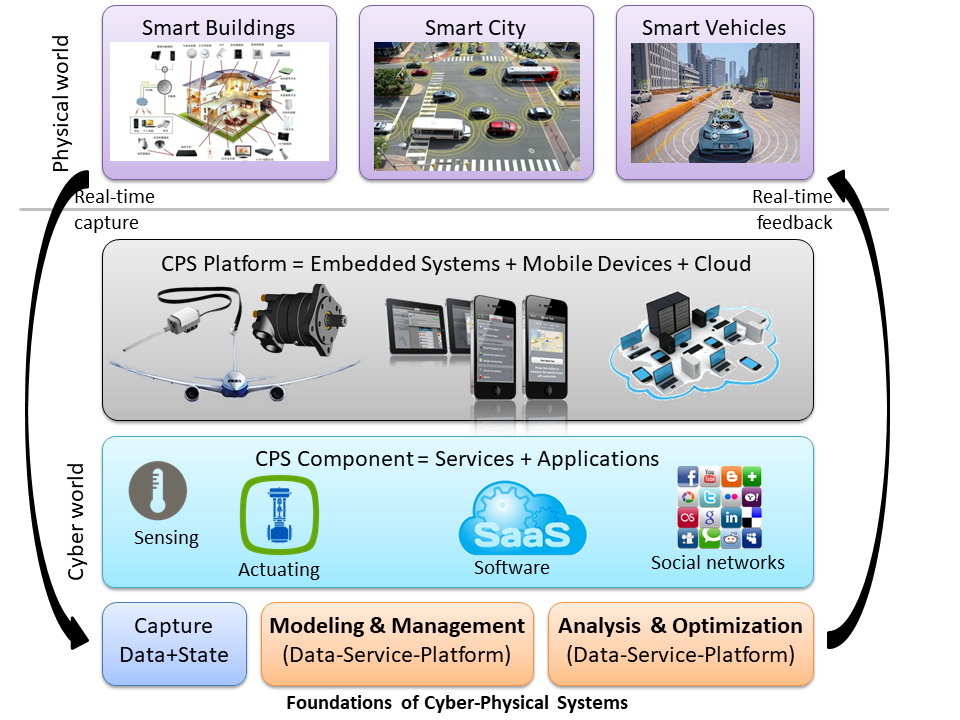
\includegraphics[width=.7\textwidth]{figures/smart-safe-cps}
\caption{Smart and safe cyber-physical systems}
\label{fig:smart-safe-cps}
\end{figure}


\paragraph{Objectives.}
My recent research has been aiming to develop innovative \emph{design, synthesis, management, validation and optimization techniques and tools}  for engineering smart and safe CPSs. In particular, my research group has been working to address two key long-term objectives:

\begin{itemize}
\item \textbf{Long-Term Objective 1}: How to \emph{design and manage} dynamically evolving smart\& safe CPSs to fulfill multi-domain requirements (e.g. consistency, extra-functional or physical)?
\item \textbf{Long-Term Objective 2}: How to \emph{guarantee or validate} that smart\& safe CPS with multi-domain requirements deliver quality of service in an open and changing environment?
\end{itemize}

\paragraph{Research environment.}
This research has been carried out in a rather unique and unconventional research environment. In 2015, I successfully acquired a Hungarian prestigious and highly selective Research Chair position funded by the Hungarian Academy of Sciences to run the \href{https://mta.hu/lendulet/az-mta-lendulet-kutatocsoport-halozata-105402}{MTA-BME Lendület Cyber-Physical Systems Research Group}. Here I was main supervisor of five PhD students, but I also provided co-supervision or strategic guidance for six other PhD students (partially affiliated to the project) who are supervised by young faculty members at the Department of Measurement and Information Systems. 
In response to the increasing direct political influence on academic institutes and research funding imposed by the Orbán Government in Hungary, I joined the Department of Electrical and Computer Engineering at McGill University as a full professor in 2016. Since then, I have been coordinating research of a virtual (trans-Atlantic) group with frequent visits of Hungarian students at McGill.

Furthermore, I was directly involved in strategically shaping proposals for European projects and training networks where IncQuery Labs Ltd was the involved partner.  Along these lines, we achieved the following major results in the past 5-6 years. 

\subsection{Secure collaborative modeling}
\paragraph{Result.} 
Cross-organizational collaboration in systems engineering projects imposes major challenges for access control management to protect the intellectual property rights (IPR) of involved parties (e.g. different vendors providing components for a system integrator). Together with C. Debreceni, M. Búr, G. Bergmann and I. Ráth, we developed a collaborative modeling framework that provides secure views with precisely defined model access to each collaborator by high-level access control policies. Our novel concepts include rule-based fine-grained access control using bidirectional transformations, property-based locking and automated model merge driven by design space exploration.

\paragraph{Impact.} 
We published seven research papers \cite{fase2016-merge,MODELS2016-access,models2017,esec-fse2017,vlhcc2018,sosym2017-mondo,ieeesw2018} at leading scientific forums (including conferences like MODELS, FASE, ESEC/FSE, VL/HCC and journals like Software and Systems Modeling and IEEE Software). Paper \cite{MODELS2016-access} received \textbf{ACM Distinguished Paper Award} at the MODELS 2016 conference, while the papers above received over 40 citations (Google Scholar). Paper \cite{vlhcc2018} carried out a user study in an industrial setting as part of the MPM4CPS EU COST Action.

\paragraph{My role.} 
I was the strategic initiator of this research line. I am the main supervisor of C. Debreceni and M. Búr who were major technical contributors of the framework. I was the site leader of the MONDO FP7 project at BME where this line of research was started, and the PI of the Lendület project which provided continuity. I helped G. Bergmann (who is an assistant professor at BME) to successfully apply to the prestigious János Bolyai Scholarship in Hungary in a related research topic. I was the Hungarian representative of the MPM4CPS EU COST Action supporting the collaboration for the user study, while the user study itself was mainly driven by A. Barisic, V. Amaral, M. Goulao (Lisbon).

\subsection{Graph queries for runtime monitoring} 
\paragraph{Result.}
We proposed different graph-based technologies for runtime monitoring purposes in smart\& safe CPS. For that purpose, we adapted (with M. Búr, G. Szilágyi and A. Vörös) existing model management and distributed graph query techniques to be deployed over a heterogeneous, decentralized execution platform with resource constraints \cite{fase2018-cps}. Furthermore, with I. Dávid and I. Ráth, we adapted the concepts of complex event processing for runtime models \cite{models2014-stream,sosym2018-cep} for stream processing. 

\paragraph{Impact.} 
We published several papers at leading conferences  \cite{fase2018-cps,nfm2018} (FASE, NASA Formal Methods) and journals \cite{sosym2018-cep}. Our paper \cite{fase2018-cps} received an \textbf{EASST Best Paper Award} at ETAPS 2018 (1 award out of over 140 papers). The MoDeS3 framework has been demonstrated at numerous industrial and other public events at BME (e.g. at the annual Researchers Night). These conceptual results have been successfully used in the MoDeS3 open demonstrator for smart and safe CPSs \cite{nfm2018} and in an initial prototype developed for the successful Hungarian start-up TeqBall.

\paragraph{My role.}
I was the main supervisor of M. Búr (PhD student at McGill) and provided strategic guidance for A. Vörös (assistant professor at BME). I contributed to the precise mathematical foundation of the results \cite{models2014-stream,sosym2018-cep}. I was the PI of the Lendület Research Group (Hungary) and a NSERC Discovery Grant (Canada). I delivered a keynote talk at Ericsson Industrial Day, at the CSCS 2016 Hungarian conference for PhD students, and several invited lectures at the DSM-TP international summer school. 

\subsection{Automated generation of consistent and diverse models}

\paragraph{Result.} 
With my students, O. Semeráth, A. Nagy, G. Szárnyas, A. Babikian, S. Pilarski, we developed a novel graph solver for automatically generating consistent and diverse graph models satisfying various structural constraints. Unlike existing approaches that map the graph generation challenge to logic solvers, our approach \cite{sosym2017-dsl,act2017,fmhe2018,fase2018-diverse,icse2018-solver,icse2019-tool} implements a refinement calculus using partial models. As such, it simultaneously provides consistency and completeness guarantees, which is a unique feature.
%Our approach (published in \cite{sosym2017-dsl,act2017,fmhe2018,fase2018-diverse,icse2018,icse2019-tool}) scales 1-2 orders of magnitude better than competitors using state-of-the-art logic solvers like Alloy (MIT) or Z3 (Microsoft Research) and its scalability is comparable to search-based techniques \cite{Soltana2017}. 
We also developed the first characterization of \emph{realistic models} in \cite{MODELS2016-metrics,fmhe2018} adapting various graph metrics from network science. By adapting graph shapes, we proposed \emph{model diversity metrics} \cite{fase2018-diverse} by which generalize and subsumes several existing coverage metrics used for testing of model transformations. We have shown that our model generator derives more diverse models than its direct competitors \cite{fase2018-diverse,fmhe2018}. 

\paragraph{Impact.} 
The news about our ICSE paper \cite{icse2018-solver} was \emph{featured on the front page of the Hungarian Academy of Sciences} (\href{http://mta.hu/english/innovation-of-hungarian-researchers-could-revolutionise-car-industry-design-technology-testing-108434}{Eng}, \href{http://mta.hu/tudomany_hirei/magyar-kutatok-eredmenye-forradalmasithatja-az-autoipari-tervezoeszkozok-teszteleset-108355}{Hun}) and shared by \emph{six major news portals in Hungary}, and I received three invitations for interviews in radio channels. Our approach (published in \cite{sosym2017-dsl,act2017,fmhe2018,fase2018-diverse,icse2018-solver,icse2019-tool}) \emph{scales 1-2 orders of magnitude better} than competitors using state-of-the-art logic solvers like Alloy (MIT) or Z3 (Microsoft Research) and its scalability is comparable to search-based techniques \cite{Soltana2017}. I also give an invited talk on this topic at the CSER 2017 conference in Montreal.

%The model generator tool \cite{icse2018,icse2019-tool} provides 1-2 orders of magnitude better scalability compared to exis
%Already the initial results for the formal validation technique for DSLs \cite{models2013} (extended later to the journal paper \cite{sosym2017-dsl}) received Best Paper Award at the IEEE/ACM MODELS 2013. 

\paragraph{My role.}
I was the sole PhD supervisor of key contributors (O. Semeráth, G. Szárnyas, A. Nagy) and MEng students (A. Babikian, S. Pilarski) of this research line. I was the first author of \cite{fmhe2018}, which presents a long-term research agenda and challenges for automated graph model generation including precise foundations. I was the PI of the Lendület project and NSERC Discovery Grant that provided funding for the involved students.

\section{Ongoing and Future Research}

\subsection{Context}

\paragraph{Motivation.} 
Digitalization is a dominating trend in engineering in initiatives like Industry 4.0 or Internet-of-Things. The concept of \emph{digital twins} (i.e. digital replica of physical assets, processes, people, places, systems) requires developing and continuously maintaining a digital representation of design documents in the form of models using a multitude of design, validation and optimization tools. The traditionally separate design and operation phases are blurred by systematically recording operational (field) data and processing it by machine learning and software engineering techniques to provide useful input for next design cycles. Decision making in autonomous CPSs (like self-driving cars, or drones) relies upon runtime models collected by a network of sensors, and fused by various artificial intelligence techniques. 

\paragraph{Main challenge.}
While innovation for digitalization is driven by software and intelligent data processing techniques; however, there is too much optimism for their fast penetration to critical CPSs (like cars, aircrafts, space) while appropriate means of quality assurance is severely lacking, especially in the presence of an increased level of automation or autonomous behavior.
 
\begin{itemize}
\item[(1)] 
While dozens of software tools are necessitated to a fully digital design of a complex CPS, quality assurance for tools and integrated tool chains is insufficient and represents a major risk for digitalization. How to trust a digital twin if one cannot trust the software tool used for designing it? Software safety standards of critical avionics systems (\href{https://standards.globalspec.com/std/1461615/rtca-do-330}{DO-330}) prescribe that only the output of a qualified tool can be trusted, and such a tool should meet the same requirements as the critical system component it designs. However, it makes tool qualification extremely costly.

\item[(2)]
Due to recent fatal accidents, the safety assurance of autonomous cyber-physical systems (like self-driving cars or autonomous drones) is still its infancy. Unfortunately, decades of verification and validation (V\&V) practices developed for traditional safety-critical software systems are not applicable to autonomous systems. Existing practices rely up exhaustive simulation for system validation, but statistical techniques do not provide sufficient level of dependability and coverage in case of extremely rare events where one combination of rare events may jeopardize safety.
\end{itemize}

\paragraph{Objectives.}
As a high-level objective, my ongoing and future research aims to increase the level of trust in digitalization for CPSs by developing systematic validation techniques for design tool chains and autonomous systems by automatically synthesizing potentially unsafe or problematic corner-cases and contextual situations. While the potential of digitalization is unquestionable, this project will mitigate its risks and negative impacts.

In particular, I am interested in novel scientific foundations and scalable software tools for 
\begin{enumerate}
\item the integration and testing of design tools used in digitalization for CPS, 
\item the system-level assurance of autonomous CPS,
\item the systematic testing for intelligent CPS driven by machine learning. 
\end{enumerate}

\subsection{Design platform for aeroderivative gas turbines}

\paragraph{Key ideas.} 
In 2018, we started a multidisciplinary collaborative research project funded by Siemens Canada and NSERC targeting a design platform for designing aeroderivative gas turbines. %With M. Rangappa, J. Dhaliwal and S. Pilarski, 
We work on innovative flexible software-as-a-service solutions to integrate various design, analysis and optimization tools driven by workflows. Moreover, we aim to develop a cloud-based solution to systematically store and query simulation results to allow fast iterations and a more agile design process. Moreover, we aim to exploit advance machine learning techniques to bring expertise gained from field data and simulated data directly to the mechanical engineers working on engine design. A follow-up project is under discussion to provide systematic testing and quality assurance for complex design tool chains.

\paragraph{My role.}
I am a co-PI of the related NSERC project (PI: M. Kokkolaras, co-PI: H. Moustapha), and the only software engineering professor in the collaboration. I am main supervisor of the three MEng students working on the project. In 2018, I was an invited speaker at the Siemens Industrial Day at ETS (Montreal), and also gave a talk about the project to graduate students.

\subsection{System-level assurance of autonomous CPS}

\paragraph{Key ideas.}
Since safety-critical autonomous vehicles need to interact with an immensely complex and continuously changing environment, their assurance is a major challenge, and upfront design time assurance is generally regarded to be practically infeasible. While systems engineering practice necessitates assurance on multiple levels,  existing research focuses dominantly on component-level assurance while neglecting complex system-level traffic scenarios.
Our research aims to address the system-level testing of the situation-dependent behavior of autonomous vehicles by combining various model-based techniques on different levels of abstraction. 

(1) Safety properties are continuously monitored in challenging test scenarios (obtained in simulators or field tests) using graph query and complex event processing techniques.  (2) To precisely quantify the coverage of an existing test suite with respect regulations of safety standards, we provide qualitative abstractions of causal, temporal, or geospatial data recorded in individual runs into situation graphs, which allows to systematically measure system-level situation coverage (on an abstract level) wrt. safety concepts captured by domain experts.  (3) Moreover, we can systematically derive new challenging (abstract) situations which justifiably lead to runtime behavior which has not been tested so far by adapting consistent graph generation techniques, thus increasing situation coverage. (4) Finally, such abstract test cases are concretized so that they can be investigated in a real or simulated context.

%\begin{enumerate}
%\item Safety properties are continuously monitored in challenging test scenarios 
%(obtained in simulators or field tests) using graph query and complex event processing techniques.  
%\item To precisely quantify the coverage of an existing test suite with respect regulations of safety standards, we provide qualitative abstractions of causal, temporal, or geospatial data recorded in individual runs into situation graphs, which allows to systematically measure system-level situation coverage (on an abstract level) wrt. safety concepts captured by domain experts. 
%\item Moreover, we can systematically derive new challenging (abstract) situations which justifiably lead to runtime behavior which has not been tested so far by adapting consistent graph generation techniques, thus increasing situation 
%coverage. 
%\item Finally, such abstract test cases are concretized so that they can be investigated in a real or simulated 
%context.
%\end{enumerate}

\subsection{Testing of data sets used for machine learning in CPS design}

\paragraph{Objectives.} Even when a large amount of field data is available as a training set, machine learning techniques provide no guarantees that this training set covers particular corner cases and rare events. We plan to devise an iterative and incremental approach which continuously evaluates a training set with respect to some coverage criteria over an abstract (graph-level) equivalence class, and then uses a graph generator (see below) to systematically derive test data for uncovered partitions of training data.

\subsection{Auto-generation of consistent, realistic, diverse and scalable models}
\paragraph{Objectives.} As a cross-domain underlying research line, we aim to develop automated synthetic graph generators with precise foundations, efficient algorithms and open-source scalable software prototype implementation to derive domain-specific graph models which are \emph{simultaneously consistent, realistic, diverse and scalable}. 
Since graphs provide key abstractions of complex information in science and technology (including  design and runtime information of complex, software-intensive CPS), auto-generated graph models can serve as test cases or benchmarking purposes, especially, in data intensive, decentralized applications.

%In a related line of research, we aim to characterize realistic engineering models 


%automated, domain-specific synthetic graph generators for the systematic validation of critical cyber-physical systems (CPS) to revolutionize 
%(1)-the testing of design tools used in digitalization for CPS, 
%(2)- the system-level assurance of autonomous CPS,
%(3)- the systematic testing for intelligent CPS driven by machine learning. 
%This will be achieved by systematically deriving rare but potentially dangerous combination of events and contextual situations captured as abstract graphs after qualitative abstractions of complex causal, temporal and spatial information. Auto-generated graphs will be simultaneously consistent, realistic, diverse and scalable with guaranteed coverage. 



\newpage

\section{Three Selected Publications with their Impact}
\lhead{Three selected publications} 

\subsection{As first author: Generic and meta-transformations}

\emph{D. Varró, A. Pataricza: Generic and meta-transformations. UML 2004} \cite{uml2004-meta}

This paper \cite{uml2004-meta} introduced the concepts of generic and meta-transformations for the first time. Generic transformations take metamodel elements as parameters or variables while meta-transformations manipulate transformations a first-class artifacts. Our result preceded the next paper on a similar topic by almost three years. After receiving significant attention from the community (currently 175 citations, VIATRA as a tool with 1500+ citations), our paper received a 10-year \textbf{Most Influential Paper Award} at the MoDELS 2014 conference, and I \emph{gave a plenary talk} on that occasion. Moreover, the first open source and Eclipse-based version of the VIATRA model transformation framework (see also e.g. \cite{sac06-vtcl,scp-2007,sosym2016-viatra-invited}) was also reported in this paper. The VIATRA framework has been used by 10+ groups worldwide and in \emph{numerous European research projects} (e.g. DIANA, DECOS, SENSORIA), and helped establish my academic reputation in the software engineering community. 

\subsection{As senior author: Scalable incremental model queries}

\emph{Z. Ujhelyi, G. Bergmann, Á. Hegedüs, Á. Horváth, B. Izsó, I. Ráth, Z. Szatmári, D. Varró:
EMF-IncQuery: An integrated development environment for live model queries. Sci. Comput. Program. 98: 80-99 (2015)} \cite{scp2015}

This paper \cite{scp2015} is the final journal version of our research line started in 2010 on scalable incremental model queries which involved six of my former PhD students. Related papers \cite{models-2010-incquery,icmt2011,ase2011-tool,ecmfa2011,models2014-iqd,scp2015,icgt2015,sosym2016-viatra-invited,models2018-tool} have been \textbf{cited over 400 times} and \cite{models2018-tool} received a \textbf{Best Tool Paper Award} at the MoDELS 2018 conference. EMF-IncQuery (now called VIATRA-Query) has become open source software framework \textbf{integrated into popular industrial tools} (Artop, Capella, Papyrus), software products in the automotive domain and in numerous European projects. It has been \emph{regularly used a baseline in performance comparisons} by leading researchers in the field, and I \emph{delivered several keynote talks} on related topics at major scientific conferences and summer schools. Finally, it served as the technological basis of \textbf{innovative products offered by IncQuery Labs Ltd., a successful Hungarian company} now with 30+ employees co-founded in 2012 with my former PhD students. 

\subsection{Last 5 years: Automated generation of consistent and diverse models}

%\emph{G. Bergmann, C. Debreceni, I. Ráth, D. Varró: Query-based access control for secure collaborative modeling using bidirectional transformations. MoDELS 2016} \cite{MODELS2016-access}

\emph{O. Semeráth, A. Nagy, D. Varró: A Graph Solver for the Automated Generation of
Consistent Domain-Specific Models. ICSE 2018} \cite{icse2018-solver}

To address various testing scenarios, we developed a novel graph solver for automatically generating consistent and diverse graph models satisfying various structural constraints. Unlike existing approaches that map the graph generation challenge to logic solvers, our approach \cite{icse2018-solver,fase2018-diverse,icse2019-tool} directly operates over partial graph models and it simultaneously provides \emph{consistency, completeness and diversity guarantees} with \emph{1-2 orders of magnitude better scalability} compared to model generators using a background logic solver (like Alloy \cite{Torlak2007} or Z3 \cite{Moura-tacas2008}). The news about our ICSE 2018 paper \cite{icse2018-solver} was \emph{featured on the front page of the Hungarian Academy of Sciences} (\href{http://mta.hu/english/innovation-of-hungarian-researchers-could-revolutionise-car-industry-design-technology-testing-108434}{Eng}) and shared by \emph{six major news portals in Hungary}, and I received three invitations for an interview in different radio channels. We wrote a related \href{https://modeling-languages.com/a-graph-solver-for-automatically-generating-consistent/}{post} for the popular blog on modeling languages.

%Our approach (published in \cite{sosym2017-dsl,act2017,fmhe2018,fase2018-diverse,icse2018,icse2019-tool}) scales 1-2 orders of magnitude better than competitors using state-of-the-art logic solvers like Alloy (MIT) or Z3 (Microsoft Research) and its scalability is comparable to search-based techniques \cite{Soltana2017}. 

%\subsection{Last 5 years: Secure views for collaborative modeling}
%
%%\emph{G. Bergmann, C. Debreceni, I. Ráth, D. Varró: Query-based access control for secure collaborative modeling using bidirectional transformations. MoDELS 2016} \cite{MODELS2016-access}
%
%\emph{C. Debreceni, G. Bergmann, I. Ráth, D. Varró: Enforcing fine-grained access control for secure collaborative
%modelling using bidirectional transformations. Software and Systems Modeling} \cite{sosym2017-mondo}
%
%
%Cross-organizational collaboration in systems engineering imposes major challenges for access control management to protect the intellectual property rights of involved parties %(e.g. different vendors providing components for a system integrator). 
%Together with C. Debreceni, G. Bergmann and I. Ráth, we proposed a collaborative modeling framework that provides secure views with precisely defined model access control to each collaborator by high-level access control policies specified by graph queries and enforced by bidirectional transformations. The original conference version of our paper \cite{MODELS2016-access} received an \textbf{ACM Distinguished Paper Award} at the IEEE/ACM MODELS 2016 conference, the main scientific venue of my research area - hereby, I included its journal extension \cite{sosym2017-mondo} to Software and Systems Modeling journal (Springer). Furthermore, we published a series of follow-up papers \cite{models2017,esec-fse2017,vlhcc2018,ieeesw2018} at leading scientific forums. As an industrial impact, most of these concept have been \textbf{adopted in the IncQuery Server for TeamWork Cloud product} \cite{models2018-tool} at IncQuery Labs Ltd. 




\newpage

%\section{List of Publications}

\newrefcontext{extref}
\printbibliography[heading=bibliography,notcategory=own,title=References]
\lhead{References} 

\newpage

\section*{List of Publications}
\lhead{List of publications} 

\begin{table}[htb]
\begin{tabular}{@{}lllll@{}}
\toprule
\textbf{Publications} & \textbf{Lifetime} (20y) & \textbf{McGill} (3y) & \textbf{Student co-author} \\ \midrule
Journals & 45 & 6 & 28 \\ \midrule
Book chapters & 9 & 1 & 6  \\ \midrule
Conferences & 68 & 16 & 54  \\ \midrule
Workshops & 33 & 2 & 20  \\ \midrule
Other & 3 & 0 & 2  \\ \midrule
Invited & 7 & 0 & N/A   \\ \midrule
Edited & 10 & 1 & N/A \\ \midrule
%PhD theses &  9 & 1 & All \\ \midrule
\bottomrule
\end{tabular}
\caption{Publication overview (Lifetime: 20 years, McGill: 3 years)}
\label{tab:publication-overview}
\end{table}


\emph{Comments to publication list:} Names of students who worked under my supervision (or co-supervision) at the time of publication are marked with \textsuperscript{*}. The first author of a paper is frequently a graduate student who made the most direct contribution to the research. The last author is typically the supervisor who signs the research program. However, other policies of authorship are also common in case of cross-institutional collaborations (e.g. alphabetical order, mixed alphabetical, etc.). 

%============= Books and Book chapters ================
\nocite{fmi2004,nagl65-2010,bpel2sal-sensoria-book,sensoria-uml,SENSORIABook:AdvancesInGT,%
mdegt2005-ggzvvv,caise2011-revised,fmic2005-pv,fmhe2018}

\addtocategory{own}{fmi2004,nagl65-2010,bpel2sal-sensoria-book,sensoria-uml,SENSORIABook:AdvancesInGT,%
mdegt2005-ggzvvv,caise2011-revised,fmic2005-pv,fmhe2018}


%============= Journal papers ================
\nocite{SCP2002,GRABATS2002j,GTVMT2003j,sosym2003-vpm,pp2003-as,FundInf2003-ghv,%
sosym2004-mc,gtvmt2004-gsv-j,gtvmt2004-vv-j,grabats2004-vfv-j,%
sosym2005-db,gramot2005-j,gramot2005-tax-j,%
sosym2005-bhtv,pngt2006-vv,gramot2006-j,hiradas2006-hvv,%
scp-2007,GT-VMT2007-hvv,gtvc2006-gkv,gtvmt2006-dpv-j,%
ijcsse08-kgv,Gonczy-safecert08,sosym2008-mtbe,%
Rath-sosym09,Bergmann-gtvmt09,%
Bergmann-sttt10,Gilmore-sosym10,eceasst2010-guided,eceasst2011-type,%
sosym2012-tools,sosym2011-cdt,sosym2011-csp,%
scp2015,ause2015,ist2015,sosym2016-trace,sosym2017-dsl,%
sosym2018-cep,sosym2016-viatra-invited,sosym2017-mondo,sosym2017-tb,act2017,sosym2018-mt,ieeesw2018} 

\addtocategory{own}{SCP2002,GRABATS2002j,GTVMT2003j,sosym2003-vpm,pp2003-as,FundInf2003-ghv,%
sosym2004-mc,gtvmt2004-gsv-j,gtvmt2004-vv-j,grabats2004-vfv-j,%
sosym2005-db,gramot2005-j,gramot2005-tax-j,%
sosym2005-bhtv,pngt2006-vv,gramot2006-j,hiradas2006-hvv,%
scp-2007,GT-VMT2007-hvv,gtvc2006-gkv,gtvmt2006-dpv-j,%
ijcsse08-kgv,Gonczy-safecert08,sosym2008-mtbe,%
Rath-sosym09,Bergmann-gtvmt09,%
Bergmann-sttt10,Gilmore-sosym10,eceasst2010-guided,eceasst2011-type,%
sosym2012-tools,sosym2011-cdt,sosym2011-csp,%
scp2015,ause2015,ist2015,sosym2016-trace,sosym2017-dsl,%
sosym2018-cep,sosym2016-viatra-invited,sosym2017-mondo,sosym2017-tb,act2017,sosym2018-mt,ieeesw2018} 

%============= Conference papers ================

\nocite{UML2002,ASE2002,ICGT2002-GHV02,ICGT2002-SC,%
esec03-bhtv,uml2003-tool,%
wicse2004-bhtv,GI2004,icgt2004-rsv,uml2004-meta,%
isas05-bvp,fase2005-eeltvv,vlhcc05-vsv,%
sac06-vtcl,sac06-plugin,isas2006-kvn,models2006-varro,icgt2006,%
agtive07-vhv,isas-2007-kv,sac2007-vb,%
icgt08-bhrv,Gonczy-mdwe08,icmt08-rbov08,Rath-vlhcc08,%
Bergmann-icmt09,Horvath-models09,Rath-models09,%
SEFM10-back-ann,models-2010-incquery,%
ase2011-dse,ase2011-mtslice,ase2011-tool,vlhcc2011,ecmfa2011,icmt2011,ServiceWave2011,%
models2012,ecmfa2012,icgt2012-ts,icst2012,tools2012,models2013,%
ase2014,models2014-iqd,models2014-stream,sle2014,csmr2014,%
icmt2015,icgt2015,%
fase2016-solver,fase2016-merge,icgt2016,MODELS2016-access,MODELS2016-bx,MODELS2016-metrics,%
esec-fse2017,models2017,adbis2017,icmt2017,%
icse2018-solver,icse2018-gamma,fase2018-diverse,fase2018-cps,models2018,vlhcc2018,nfm2018,models2018-tool,%
icse2019-tool} 

\addtocategory{own}{UML2002,ASE2002,ICGT2002-GHV02,ICGT2002-SC,%
esec03-bhtv,uml2003-tool,%
wicse2004-bhtv,GI2004,icgt2004-rsv,uml2004-meta,%
isas05-bvp,fase2005-eeltvv,vlhcc05-vsv,%
sac06-vtcl,sac06-plugin,isas2006-kvn,models2006-varro,icgt2006,%
agtive07-vhv,isas-2007-kv,sac2007-vb,%
icgt08-bhrv,Gonczy-mdwe08,icmt08-rbov08,Rath-vlhcc08,%
Bergmann-icmt09,Horvath-models09,Rath-models09,%
SEFM10-back-ann,models-2010-incquery,%
ase2011-dse,ase2011-mtslice,ase2011-tool,vlhcc2011,ecmfa2011,icmt2011,ServiceWave2011,%
models2012,ecmfa2012,icgt2012-ts,icst2012,tools2012,models2013,%
ase2014,models2014-iqd,models2014-stream,sle2014,csmr2014,%
icmt2015,icgt2015,%
fase2016-solver,fase2016-merge,icgt2016,MODELS2016-access,MODELS2016-bx,MODELS2016-metrics,%
esec-fse2017,models2017,adbis2017,icmt2017,%
icse2018-solver,icse2018-gamma,fase2018-diverse,fase2018-cps,models2018,vlhcc2018,nfm2018,models2018-tool,%
icse2019-tool}

\nocite{dasc2010-hvs,Daboczi-AWSN2013,dasc2014}
\addtocategory{own}{dasc2010-hvs,Daboczi-AWSN2013,dasc2014}

%============= Workshop papers ================

\nocite{GRATRA2000,DDECS2000,WTUML01,%
edcc2002-svp,FMOODS2002,AGT2002,%GRABATS2002,GTVMT2002,
cbse03-bhtv,DDECS2003-tvp,csduml2003,%%grabats2004-vfv,gtvmt04-vv,gtvmt04-gsv,
mtip2005,%gramot2005-tax,gramot2005-adapt,gramot2006-vvs,
cmt2006,wsmate2006,dspd2006-rv,models2006-edu,%pngt2006-vv,gtvc2006-gkv,gtvmt06-dpv,
efts-2007-kgv,%GT-VMT2007-hvv,
gramot08-borvv,%Gonczy-safecert08,%Bergmann-gtvmt09,
SEFM10ToolDemo-back-ann,%eceasst2010-guided,
ocl2012,amt2012-query,
Kolovos-bigmde2013,Izso-bigmde2013,%
bigmde2014,cmseba2014,mpm2014,oss4mde2014,vao2014,%
staf2015-project,ttc2015,gemoc2015,%
BX2016,STAF-proj-2016,commitmde2016,%
commitmde2017}

\addtocategory{own}{GRATRA2000,DDECS2000,WTUML01,%
edcc2002-svp,FMOODS2002,AGT2002,%GRABATS2002,GTVMT2002,
cbse03-bhtv,DDECS2003-tvp,csduml2003,%%grabats2004-vfv,gtvmt04-vv,gtvmt04-gsv,
mtip2005,%gramot2005-tax,gramot2005-adapt,gramot2006-vvs,
cmt2006,wsmate2006,dspd2006-rv,models2006-edu,%pngt2006-vv,gtvc2006-gkv,gtvmt06-dpv,
efts-2007-kgv,%GT-VMT2007-hvv,
gramot08-borvv,%Gonczy-safecert08,%Bergmann-gtvmt09,
SEFM10ToolDemo-back-ann,%eceasst2010-guided,
ocl2012,amt2012-query,
Kolovos-bigmde2013,Izso-bigmde2013,%
bigmde2014,cmseba2014,mpm2014,oss4mde2014,vao2014,%
staf2015-project,ttc2015,gemoc2015,%
BX2016,STAF-proj-2016,commitmde2016,%
commitmde2017}

%============= Invited papers ================

\nocite{easst2006-etv,Wirsing-isola08,agtive07-toolcontest,models09-edu,csmr2012-invited,sofsem2016-invited,pame2015}
\addtocategory{own}{easst2006-etv,Wirsing-isola08,agtive07-toolcontest,models09-edu,csmr2012-invited,sofsem2016-invited,pame2015}

%============= Edited proceedings ================

\nocite{gtvmt2006,icgt2006-grabats,grabats2010,agtive2011,amt2012,fase2013,icmt2014,staf2015-ds,sle2016,staf2016-ws}
\addtocategory{own}{gtvmt2006,icgt2006-grabats,grabats2010,agtive2011,amt2012,fase2013,icmt2014,staf2015-ds,sle2016,staf2016-ws}

%============= End of own papers ================

\defbibfilter{books}{type=book or type=incollection or type=inbook}

%\defbibfilter{conf}{type=inproceedings and notkeyword={invited}}

\newrefcontext{bref}
\printbibliography[heading=subbibliography,filter=books,category=own,title=Books and Book Chapter (Total: 9)]

\newrefcontext{jref}
\printbibliography[heading=subbibliography,category=own,type=article,notkeyword={workshop},notkeyword={invited},title=Refereed Journals incl. Electronic Journals (Total: 45)]

\newrefcontext{cref}
\printbibliography[heading=subbibliography,category=own,notkeyword={invited},notkeyword={other},notkeyword={workshop},type=inproceedings,title=Peer Reviewed Conference Papers (Total: 69)]

\newrefcontext{oref}
\printbibliography[heading=subbibliography,category=own,keyword={other},type=inproceedings,title=Other Conference Papers (Total: 3)]

\newrefcontext{wref}
\printbibliography[heading=subbibliography,category=own,keyword={workshop},type=inproceedings,title=Refereed Workshop Papers (Total: 33)]

\newrefcontext{iref}
\printbibliography[heading=subbibliography,category=own,keyword={invited},title=Invited Papers (Total: 7)]

\newrefcontext{eref}
\printbibliography[heading=subbibliography,category=own,type=proceedings,title=Edited Volumes (Total: 10)]

%\newrefsection%[bib/external.bib]
%\citereset
%\newrefcontext[sorting=nty]


%\newrefcontext{cref}
%\printbibliography[heading=subbibliography,type=inproceedings,title=Peer Reviewed Conference Papers (Total: 69)]

%\end{refsection}


%
%For most top conferences, the acceptance rate is published which is typically below 33\%.  


\begin{refsection}
\newrefcontext[labelprefix=B]
  \nocite{fmi2004,nagl65-2010,bpel2sal-sensoria-book,sensoria-uml,SENSORIABook:AdvancesInGT,mdegt2005_ggzvvv,caise2011-revised,fmic2005_pv,fmhe2018}
\printbibliography[title=Books and Book Chapter (Total: 9)]
\end{refsection}


\begin{refsection}
\newrefcontext[labelprefix=J]
  \nocite{SCP2002,GRABATS2002j,GTVMT2003j,sosym2003_vpm,pp2003_as,FundInf2003_ghv,%
sosym2004_mc,gtvmt2004-gsv-j,gtvmt2004-vv-j,grabats2004-vfv-j,%
sosym2005_db,gramot2005-j,gramot2005-tax-j,%
sosym2005_bhtv,pngt2006-vv,gramot2006-j,hiradas2006-hvv,%
scp-2007,GT-VMT2007-hvv,gtvc2006-gkv,gtvmt2006-dpv-j,%
ijcsse08-kgv,Gonczy-safecert08,sosym2008-mtbe,%
Rath-sosym09,Bergmann-gtvmt09,%
Bergmann-sttt10,Gilmore-sosym10,eceasst2010-guided,eceasst2011-type,%
sosym2012-tools,sosym2011-cdt,sosym2011-csp,scp2015,ause2015,ist2015,sosym2016-trace,sosym2017-dsl,sosym2018-cep,sosym2016-viatra-invited,sosym2017-mondo,sosym2017-tb,act2017,sosym2018-mt,ieeesw2018} 
\printbibliography[title=Refereed Journals incl. Electronic Journals (Total: 45)]
\end{refsection}
 
\begin{refsection}
\newrefcontext[labelprefix=C]
  \nocite{UML2002,ASE2002,ICGT2002-GHV02,ICGT2002-SC,%
esec03_bhtv,uml2003_tool,%
wicse2004_bhtv,GI2004,icgt2004_rsv,uml2004_meta,%
isas05_bvp,fase2005_eeltvv,vlhcc05_vsv,%
sac06_vtcl,sac06_plugin,isas2006_kvn,models2006-varro,icgt2006,%
agtive07-vhv,isas-2007-kv,sac2007-vb,%
icgt08-bhrv,Gonczy-mdwe08,icmt08-rbov08,Rath-vlhcc08,%
Bergmann-icmt09,Horvath-models09,Rath-models09,%
SEFM10:back-ann,models-2010-incquery,%
ase2011-dse,ase2011-mtslice,ase2011-tool,vlhcc2011,ecmfa2011,icmt2011,ServiceWave2011,%
models2012,ecmfa2012,icgt2012-ts,icst2012,tools2012,models2013,%
ase2014,models2014-iqd,models2014-stream,sle2014,csmr2014,%
icmt2015,icgt2015,%
fase2016-solver,fase2016-merge,icgt2016,MODELS2016-access,MODELS2016-bx,MODELS2016-metrics,%
esec-fse2017,models2017,adbis2017,icmt2017,%
icse2018-solver,icse2018-gamma,fase2018-diverse,fase2018-cps,models2018,vlhcc2018,nfm2018,models2018-tool,%
icse2019-tool} 
\printbibliography[title=Peer Reviewed Conference Papers (Total: 69)]
\end{refsection}

\begin{refsection}
\newrefcontext[labelprefix=O]
  \nocite{dasc2010-hvs,Daboczi-AWSN2013,dasc2014}
\printbibliography[title=Other Conference Papers (Total: 3)]
\end{refsection}


\begin{refsection}
\newrefcontext[labelprefix=W]
  \nocite{GRATRA2000,DDECS2000,WTUML01,%
edcc2002_svp,FMOODS2002,AGT2002,%GRABATS2002,GTVMT2002,
cbse03_bhtv,DDECS2003_tvp,csduml2003,%
%grabats2004_vfv,gtvmt04_vv,gtvmt04_gsv,
mtip2005,%gramot2005_tax,gramot2005_adapt,gramot2006-vvs,
cmt2006,wsmate2006,dspd2006_rv,models2006-edu,%pngt2006-vv,gtvc2006-gkv,gtvmt06_dpv,
efts-2007-kgv,%GT-VMT2007-hvv,
gramot08-borvv,%Gonczy-safecert08,
%Bergmann-gtvmt09,
SEFM10ToolDemo:back-ann,%eceasst2010-guided,
ocl2012,amt2012-query,%
Kolovos-bigmde2013,Izso-bigmde2013,%
bigmde2014,cmseba2014,mpm2014,oss4mde2014,vao2014,%
staf2015-project,ttc2015,gemoc2015,%
BX2016,STAF-proj-2016,commitmde2016,%
commitmde2017}
\printbibliography[title=Refereed Workshop Papers (Total: 33)]
\end{refsection}
  

\begin{refsection}
\newrefcontext[labelprefix=I]
  \nocite{easst2006-etv,Wirsing-isola08,agtive07-toolcontest,models09-edu,csmr2012-invited,sofsem2016-invited,pame2015}
\printbibliography[title=Invited Papers (Total: 7)]
\end{refsection}

\begin{refsection}
\newrefcontext[labelprefix=E]
  \nocite{gtvmt2006,icgt2006-grabats,grabats2010,agtive2011,amt2012,fase2013,icmt2014,staf2015-ds,sle2016,staf2016-ws}
\printbibliography[title=Edited Volumes (Total: 10)]
\end{refsection}

\end{document}
